\documentclass[a4paper]{article}

\usepackage[utf8]{inputenc}
\usepackage[DIV=18]{typearea}
\usepackage{microtype}
\usepackage{mathtools, amssymb, bm}
\usepackage{parskip}
\usepackage{float}
\usepackage[shortlabels]{enumitem}
\usepackage[colorlinks=true]{hyperref}
\hypersetup{linktoc=all}

\title{4}
\date{}

\begin{document}
\maketitle
\section{Paper Details}
\begin{description}
	\item[Title] Text mining using nonnegative matrix factorization and latent semantic analysis
	\item[Authors] {Ali Hassani}, {Amir Iranmanesh}, {Najme Mansouri}
	\item[Venue] \href{https://link.springer.com/journal/521}{Neural Computing and Applications}, Volume 33
	\item[Year of Publication] 2021
	\item[URL] \url{https://link.springer.com/article/10.1007/s00521-021-06014-6}
	\item[Problem] The paper proposes an algorithm for Text Clustering which is a Natural Language Processing problem involving grouping a collection of textual documents into clusters based on their content's similarity. 
	\item[Subproblem involving NMF] The paper uses NMF for \textbf{Feature Extraction}, Latent semantic analysis (LSA) for dimension reduction and deterministic K-means algorithm for clustering. Usage of NMF also decreases dimensionality of the data.
	\item[Terminology] 
	A \emph{term} is a unit which could be a word or combination of words of the language.

	A matrix of concern is the \emph{term-document matrix} $X \in \mathbb{R}^{n\times m}$ which is obtained after processing the matrix which stores the frequency of a term ($m$ different terms) of a particular document ($n$ available documents) in that row as shown in the below figure from the same paper. The processing step involves stemming (reduces words to their stems) and weighting (applying weights to terms based on their frequency)
	\begin{figure}[H]
	\centering
	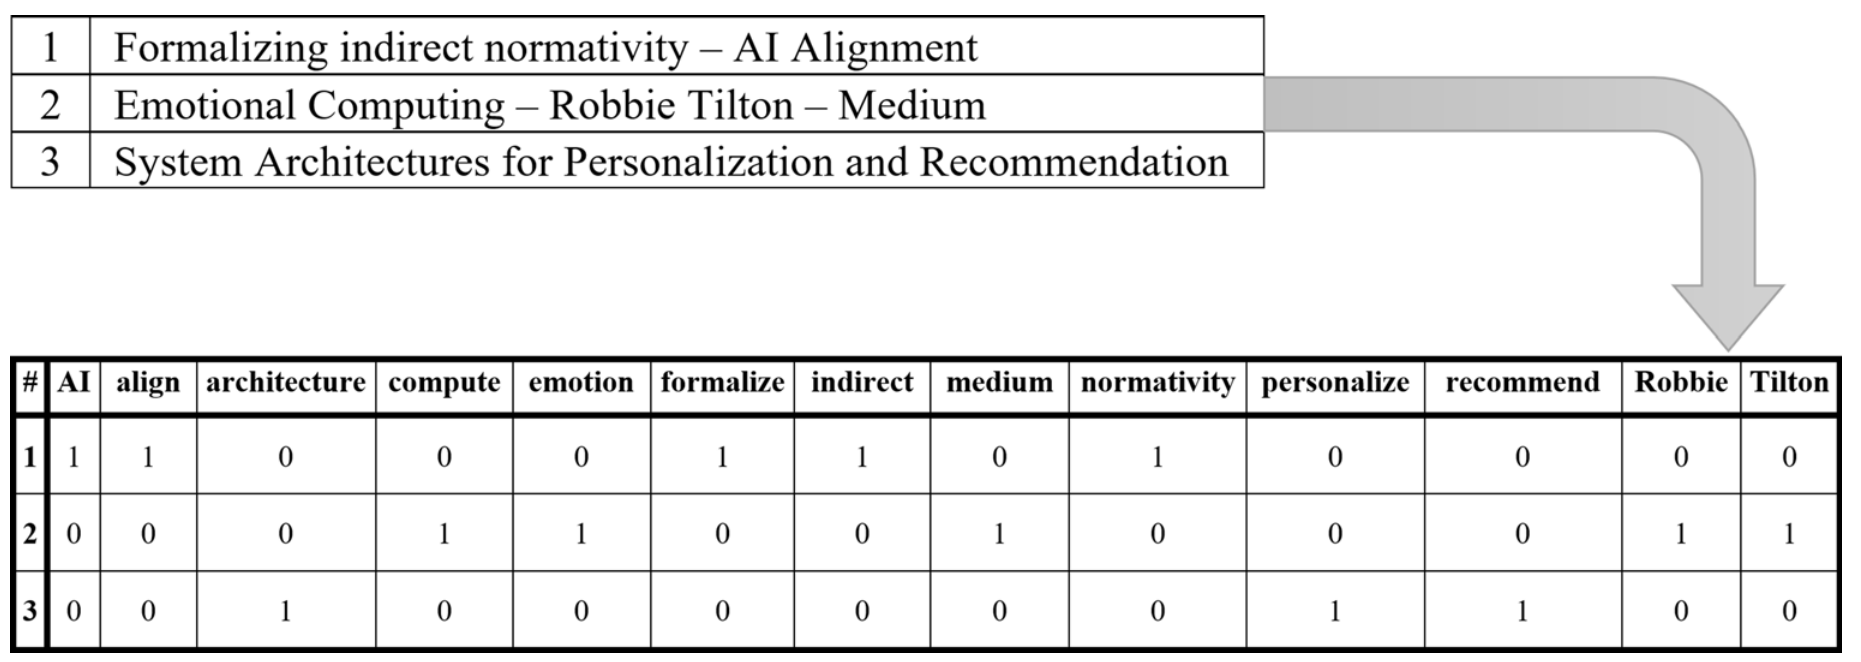
\includegraphics[width=\linewidth]{../media/Q3 count matrix.png}
	\end{figure}
	\item[Solution of the subproblem involving NMF] Feature Extraction involves creating a more suitable feature space for text clustering. This is done by separating the terms into groups and then combining each group's term vectors into new feature vectors.
	Mathematically, $\|X-WH\|_F$ is minimised such that $W\in\mathbb{R}^{n\times p}, R\in\mathbb{R}^{p\times m}\text{ and }W,H \geq 0$.
	\item[Significance of the Dictionary and its coefficients] 
	After the optimisation, $W$ represents the dictionary and $H$ gives the dictionary coefficients. $H$ is used in order to group terms together into $p$ categories and then represent each such category with a feature vector whereas an initial feature vector of each term is given by linear combination of columns of $W$ according the the dictionary coefficients. Then for each group these initial feature vectors are taken and new feature vectors are generated.
\end{description}
\end{document}